\chapter{Diferents mides de Train i diccionaris}
A continuació es fan varies proves canviant mides i analitzant si els resultats milloren o empitjoren
\section{Canviant mida del conjunt test}
A vegades pot ser interessant veure quantes mostres són necessàries per aconseguir un entrenament satisfactori. La prova de l’apartat anterior s’havia fet amb un 20\% de les mostres pel test i el 80\% restant pel training. Ara, en canvi, es realitzen diferents execucions, cada una amb una proporció traint/test diferent. 

Com bé es veu al gràfic inferior, a mesura que hi ha més mostres al test, i per tant menys al training, les prediccions tendeixen a ser pitjors. És un resultat esperat, al cap i a la fi com més dades es tingui per aprendre, més fàcil serà fer una predicció d’una nova mostra. 

El punt interessant a comentar és que s’ha de reduir molt la mida de les mostres de training fins aconseguir unes prediccions bastant més dolentes que l’original. Es veu que destintant només el 10\% de les mostres al training, es segueix aconseguint un accuracy per sobre del 70\%. És quan ja es destinen només un 2\% de les mostres que els resultats comencen a empitjorar.

La figura ~\ref{fig:test_size} mostra els resultats esmentats
\begin{figure}[h]
    \centering
    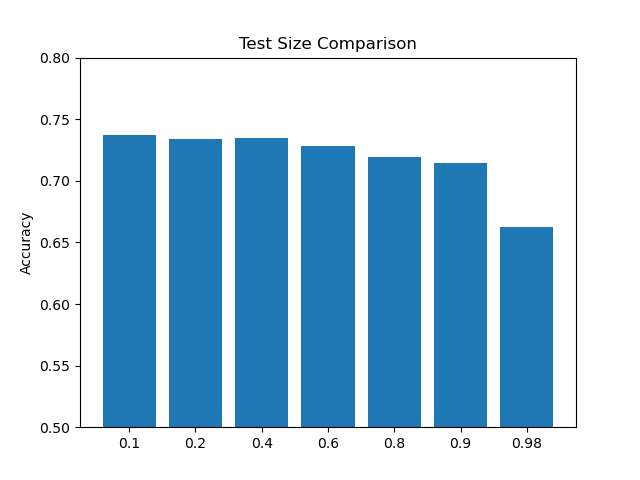
\includegraphics[height=7cm,keepaspectratio]{images/image3.png}
    \caption{Diferents mides del conjunt Test}
    \label{fig:test_size}
\end{figure}
\section{Canviant mida diccionari}
Una altra manera de veure la quantitat d’informació necessària per fer bones prediccions és limitant la mida del diccionari. És a dir, limitar la quantitat de paraules que pot aprendre el model. Com també és d’esperar, les prediccions empitjoren a mesura que hi ha menys paraules al diccionari. 

Ara, si més no, s’aconsegueix mantenir uns bons resultats tot i tenir el diccionari a l’1\% de la seva mida original. És només quan la mida baixa del 0.2\% que l’accuracy ja és inferior al 65\%.

La figura \ref{fig:dic_size} mostra els resultats esmentats.
\begin{figure}[ht]
    \centering
    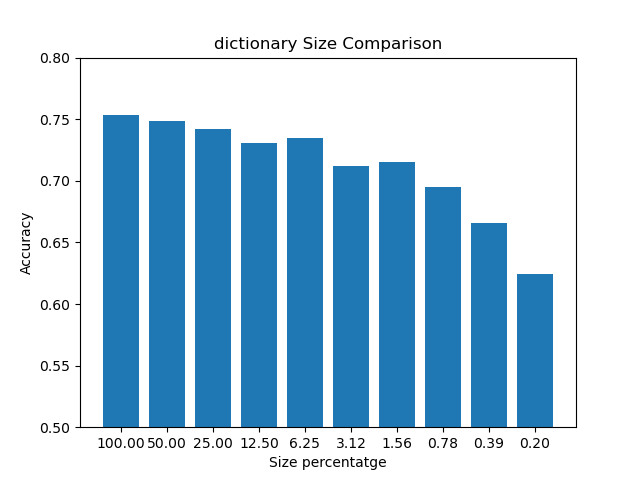
\includegraphics[width=\textwidth,height=\textheight,keepaspectratio]{images/image4.png}
    \caption{diferents mides de diccionari}
    \label{fig:dic_size}
\end{figure}
\section{Més mostres sense augmentar el diccionari}
Una última prova que s’ha fet és augmentar la mida del conjunt traint però mantenir una mida fixa del diccionari. 

Els resultats són els mateixos quan la mida del diccionari es petita. Tot i ampliar les mostres, quan el diccionari està ple, les noves mostres no es poden analitzar al complet i per tant no aporten gaire informació al model. En canvi, quan es permet una mida gran del diccionari, triga més a arribar al punt on no hi ha millora.
